\documentclass{article}
\usepackage[margin=1.5cm,bottom=2cm]{geometry}
\usepackage{fancyhdr}
\usepackage{graphicx}
\usepackage{amsmath}
\usepackage{enumitem}
\pagestyle{fancy}

\begin{document}
\fancyhead[L]{ 
\includegraphics[width=2cm]{au_logo.png} }
\fancyhead[R]{PHYS 4220: Computational Physics}
\fancyfoot[C]{\thepage}
\vspace*{0cm}
\begin{center}
	{\LARGE \textbf{Project 1}}\\
	\vspace{0.25cm}
	{\Large Two Balls In One Dimension with Gravity}
	
	{\Large Due: Friday, October 16}
\end{center}

\newcommand{\textbook}{\textit{Giordano}}

\section*{Overview}
In this project, you will consider the system of two balls bouncing in one dimension under the influence of gravity. The balls are subject to collisions with the ground and with each other. You will assume that every collision is perfectly elastic, so that energy is always conserved, and momentum is conserved immediately before and after any collision. Under certain conditions, this arrangement leads to chaotic motion.

\begin{figure}[ht]
	\centering
	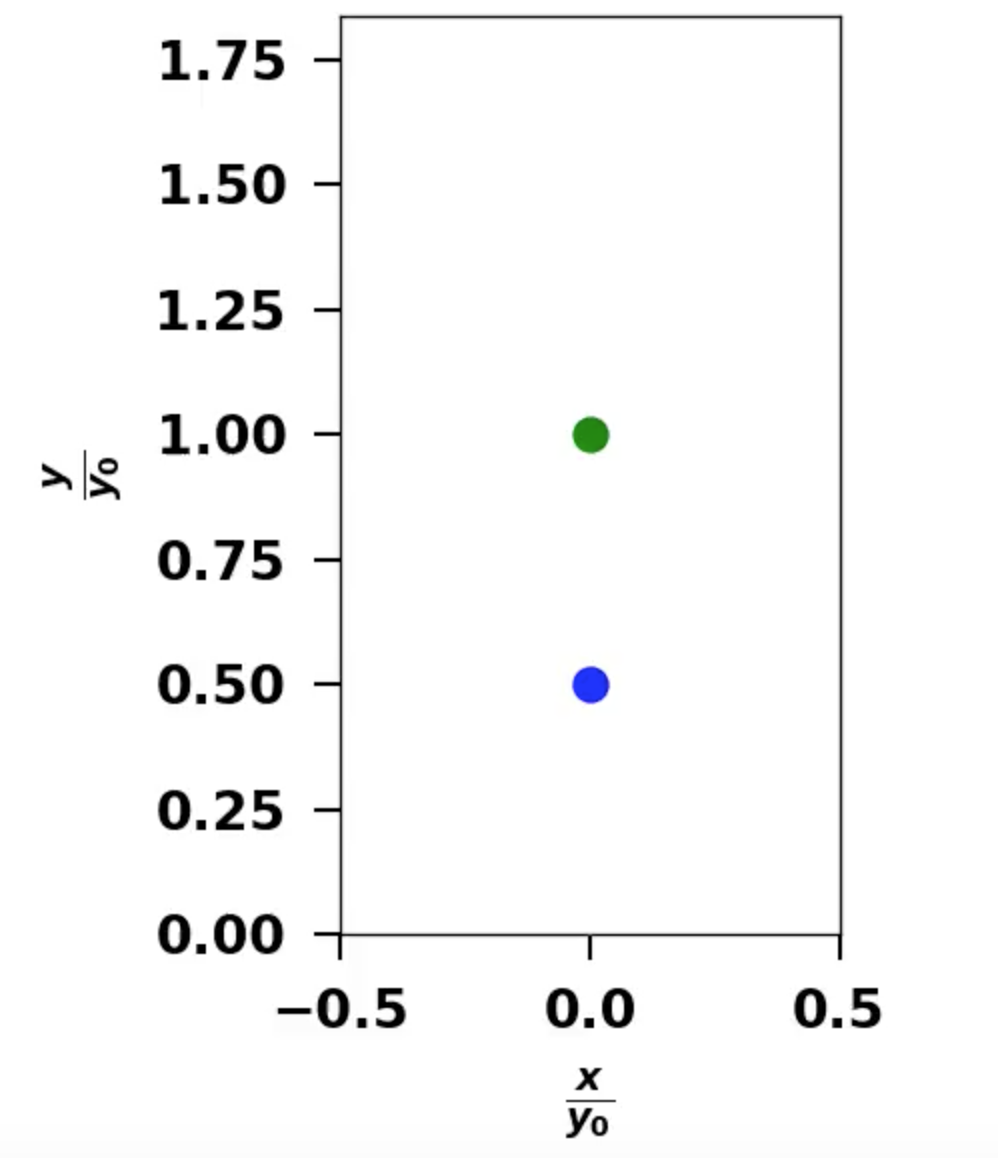
\includegraphics[width=5cm]{screen_grab.png}
\end{figure}

\section*{Setup}
\begin{itemize}
	\item Ball 1 starts from rest at some initial height $y_{1,i}$, ball 2 starts from rest at some initial height $y_{2,i}>y_{1,i}$.
	\item Ball 1 has mass $m_1$, ball 2 has mass $m_2$
	\item Each ball is subject to a constant gravitational force in the $-\hat{y}$ direction $F=-mg\hat{y}$.
	\item The balls may collide with one another. They do so elastically, such that both momentum and kinetic energy are conserved.
	\item The lower ball (ball 1) may collide with the ground $(y=0)$. Treat this as an elastic collision between the ball and an object of infinite mass.
\end{itemize}

Write a program which calculates the trajectory (velocity and position) of each ball as a function of time. You will do this for several different values of the mass ratio $m_2/m_1$.

\section*{Analysis}
Do the following for three different values of the mass ratio $r$: $|r|<1, r=1,r>1$
\begin{itemize}
	\item Plot the trajectory of each ball ($y$ vs $t$) along with the kinetic, potential, and total energy.
	\item Plot the trajectory of each ball in phase space ($y$ vs $v$)
	\item Construct the Poincar\'e section by plotting $y_2$ vs $v_2|_{y_1=0}$ (plot the phase space trajectory of the second ball for points when the first ball contacts the ground).
\end{itemize}


\end{document}